%%% Local Variables:
%%% TeX-master: "AbilityMaster"
%%% End:%%% Local Variables:
%%% TeX-master: "master"
%%% End:

\chapter{Potentive entailment --- Attribution and Witnessing}
\label{cha:potent-infer-attr}

\begin{note}[Overview]
  In this chapter focuses on understanding potentive entailment, potentive entailment with respect to (specific) abilities, and how potentive entailment with respect to (specific) abilities is used in the cases of interest.
\end{note}

\begin{note}[Plan for chapter]
  The plan for the chapter is as follows:
  \begin{itemize}
  \item Potentive entailment.
  \item Two ways in which potentive entailment may be used --- \AR{} and \WR{}.
  \item Differences between \AR{} and \WR{}.
  \item (Possibly) further notes on \WR{}.
  \end{itemize}
\end{note}




\section{Potentive entailment}
\label{sec:potentive-entailment}

\begin{note}[Potentive entailment]
  A potentive entailment is an entailment of the form:
  \begin{enumerate}
  \item In order for there to be potential for some event \(e\) to be witnessed, \(\psi\) must (already) be the case.
  \end{enumerate}
  Intuitively, there is potential for some event \(e\) to be witnessed if there are preconditions for witnessing that must been met, and the potentive entailment identifies \(\psi\) as some such precondition that has been met.

  Term this `potentive entailment' as consequent of the entailment follows from the `potential' construct of the antecedent.
  
  For example, there is potential for Smith to travel to London in time for tomorrows meeting.
  So, there is an aeroplane set to depart no later than midnight tonight for which Smith may purchase a ticket, and so on.
  

  This is `local' entailment.
  It does not look for necessary conditions for an event.
  For example, private jet.
  Given the way things are, no private jet.

  So, hard to determine whether a potentive entailment holds in general.
  May be some exception.

  For present purposes, there is potential for some event to be witnessed.

  Specially, the events of interest are an agent reasoning from some premises to a conclusion.

  \begin{enumerate}
  \item\label{PE:ability:event} As there to be potential for an event of S proving \(\phi\) to be witnessed, \(\psi\) must (already) be the case.
  \end{enumerate}

  Example.

  Finally, change of focus to the agent rather than the potential event.
  Potential for an event of \dots to be witnessed, rewrites to S has the ability to \dots

  \begin{enumerate}
  \item\label{PE:ability:agent} S has the (specific) ability to V that \(\phi\), so \(\psi\) must (already) be the case.
  \end{enumerate}

  Remains an instance of potentive entailment.

  Two important instances.
  \begin{enumerate}
  \item Conclusion is the case.
  \item Support for premises.
  \end{enumerate}

  Given that~\ref{PE:ability:event} and~\ref{PE:ability:agent} we avoid the need for an understanding of ability.
  Some worries about what it is for there to be a potential event.
  Suitable analysis may depend on ability, or perhaps ability is analysed in terms of potential events.

  In short, while~\ref{PE:ability:agent} is natural, and our preferred statement, \ref{PE:ability:event} is equivalent.
  Therefore, we will understand the use of potentive entailments involving ability in terms of potential events, rather than on the basis of any particular understanding of ability.
\end{note}

\begin{note}[Examples]
  Simple instances of the potentive entailment involve factive verbs, in which the relevant fact holds independently of whether the verb is witnessed.
  \begin{itemize}
  \item Sam has the ability to show that \(19\) is a prime number.
  \item Taylor has the ability to derive Transposition.
  \item Jesse has the ability to \dots
  \end{itemize}

  Note also that the verb does not need to involve some reasoning.
  \begin{itemize}
  \item Corey has the ability to see there is a zebra in the pen.
  \item X has the ability to hear that there is a waterfall nearby.
  \end{itemize}
\end{note}

\begin{note}[Breaking things down]
\begin{quote}
  \begin{enumerate}
  \item There is a potential event in which \emph{S} \emph{V}s that \(\phi\).
  \item \emph{S} has the ability to \emph{V} that \(\phi\).
  \end{enumerate}
  \end{quote}
  We have
  \begin{itemize}
  \item Some result of the verb.
  \item A verb.
  \item Modal, ability.
  \item An agent.
  \end{itemize}
  The two differ primarily in terms of the modal.
\end{note}

\begin{note}[Potentive]
  The potentive is straightforward to analyse.

  Fairly clear understanding of event semantics.

  Here, existential quantification over events is replaced by a modal.

  This requires some non-standard existential, but we're not too interested in providing an analysis suitable for semantics.
\end{note}


\begin{note}[Understanding potentive entailment]
  The key parts of the entailment are the relation between ability and the verb.

  Certain things must be true in order for the verb.
  These are the things which are obtained by the potentive entailment.

  In the case of reasoning, note that there must be premises from which the agent works from.
\end{note}

\begin{note}[Observation in terms of prop/dox]
  One way to view this is that if the agent has information, then the agent may infer that they have propositional support for the conclusion which may be turned in to doxastic support.
\end{note}

\begin{note}[Ability]
  Our understanding of ability is basically the same as potentive.

  Ability functions as an equivalent quantifier.

  Specific reading of ability.
  \textcite{Hackl:1998tt} distinguishes:
  {
    \small
    \begin{enumerate}
    \item John is able be a tall (in view of the evidence available).\hfill \emph{epistemic}
    \item John is able to listen to punk rock.\hfill \emph{deontic: ``allowed-to-do''}
    \item John is able to be married, according to the law.\hfill \emph{deontic: ``allowed-to-be''}
    \item John is able to jump higher than Bill.\hfill \emph{ability}
    \item John is able to see Mary from where he is standing.\hfill \emph{opportunity}
    \end{enumerate}
  }
  Only the last two readings seems natural, but all work if `able to' is read as `can'.

  We're interested in what \citeauthor{Hackl:1998tt} terms `opportunity'.
\end{note}

\begin{note}[Some formal stuff]
  \[(\text{Able}(s,e) \land (V(e) \land \text{agent} = s \land \text{result}(e) = \phi))\]
  There is some event \(e\), such that \emph{s} is able to bring about, and \(e\) consists of \emph{s} \emph{V}ing with the result that \(\phi\).

  The quantification here is somewhat familiar to Lewis' counterpart theory.

  Understand ability as relating the agent directly to an event.
  Alternative it to take a truth value.
  \((\text{Able}(s,\exists (V(e) \land \text{agent} = s \land \text{result}(e) = \phi))\).

  Close to having a possible world with \(\phi\) and accessibility relation.
  Interpret the non-standard existential in this way, if it helps.
  There is some possible world and some event in that world, such that the agent at the world of evaluation is able to perform the event witnessed at the possible world.

  In both cases, it's the role of the event.

  \begin{figure}[h]
    \begin{subfigure}{.5\textwidth}
      \centering
      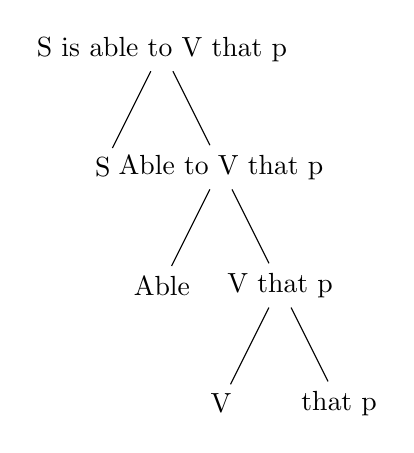
\begin{tikzpicture}[
        ]
        \node{S is able to V that p}
        child {node {S}}
        child {node {Able to V that p}
          child {node {Able}}
          child {node {V that p}
            child {node {V}
            }
            child {node {that p}
            }
          }
        };
      \end{tikzpicture}
    \end{subfigure}
    %
    \begin{subfigure}{.5\textwidth}
      \centering
      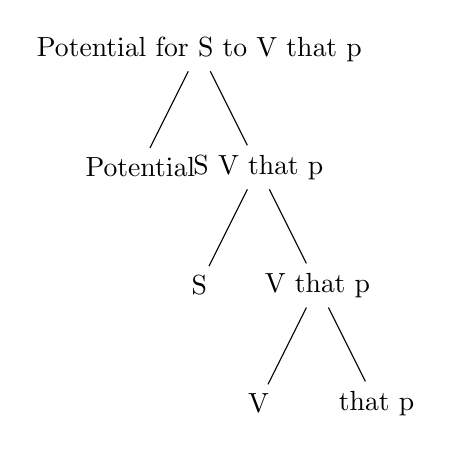
\begin{tikzpicture}[
        ]
        \node{Potential for S to V that p}
        child {node {Potential}}
        child {node {S V that p}
          child {node {S}}
          child {node {V that p}
            child {node {V}
            }
            child {node {that p}
            }
          }
        };
      \end{tikzpicture}
    \end{subfigure}
  \end{figure}
\end{note}

\begin{note}[The entailment]
  Take some arbitrary witnessing event.
  If \(\psi\) follows from the (arbitrary) witnessing event, then we have an instance of the potentive entailment.

  Pretty much the same as reasoning with existentials.
\end{note}

\begin{note}[Expanding the event]
  The description of the witnessing event given is minimal.
  Still, simply add in more detail as desired.
\end{note}

\begin{note}[Specific abilities]
  Applies to specific abilities, as the entailment appeals to a witnessing event.
  Analogue holds with respect to general abilities.

  General example:
  \begin{itemize}
  \item Sam has the ability to reason with the rules of chess.
  \end{itemize}
  Infer that there is a body of rules governing chess.
  If there are no rules governing chess, then the agent does not have the ability to reason with those (non-existing) rules.

  Not an instance of the potentive entailment, as this doesn't follow from what is required from a witnessing event.

  Similarly, it may be that there is an entailment from general to specific.
  \begin{itemize}
  \item If general, then specific.
  \end{itemize}
  For example, understand the general ability distributively.
  Again, not an instance of the potentive entailment, as this doesn't follow from what is required from a witnessing event.
\end{note}

\begin{note}[Paraphrasing (footnote)]
  Various paraphrases are available.
  \begin{itemize}
  \item Corey can see there is a zebra in the pen.
  \end{itemize}
  `Can' introduces the complexity that the agent may be witnessing.
  For example, we observe an excited look appear on Corey's face as they look into the pen.
  `Ah, Corey can see a zebra in the pen.'
  Corey isn't exited because they have the ability to see a zebra in the pen, rather Corey is excited because they are seeing a zebra.
\end{note}

\begin{note}[Restriction on instances of potentive entailment]
  We're interested in certain examples as the agent has all of the resources required, so to speak.

  To illustrate, place the reasoning examples behind a conditional.
  \begin{itemize}
  \item If you teach Sam \dots [factoring method], then Sam will have the ability to show that \(19\) is a prime number.
  \end{itemize}
  Intuitively, this is the result of assuming that some additional property holds of the agent.
  Hence, \(\alpha(s) \rightarrow \dots\).
  For, \(\alpha(s)\) will allow the attribution of ability to be true.
\end{note}

\begin{note}[Reasoning and premises]
  Important to note is that in cases of reasoning, the potentive entailment may be applied to obtain the availability of premises.

  The difference is the role of these premises.
\end{note}

\begin{note}[Two instances of potentive entailment]
  We get premises and conclusion.

  Here, the important thing is that if the agent doesn't already have the basics, then something further would need to be the case for there to be a potential event.

  Admittedly, there is no clear line.
  For, there are ways to expand the event.

  Example, lighting a match.
  Have match and matchbox in hand.
  Have matchbox.
  Matchbox is in a draw.
  Etc.

  Resolved by placing constraints on the event.
\end{note}

\begin{note}[Moving on to a more detailed understanding]
  How exactly the event works.
\end{note}

\section{\AR{} and \WR{}}
\label{sec:ar-wr}

\begin{note}[Overview]
  Interest is in how potentive entailment is used.

  A clearer understanding of \AR{} and \WR{}.

  The significant difference is with reasoning.
  \AR{} uses (a variation of) the potentive entailment to obtain support.
  \WR{} uses information obtained by the potentive entailment to obtain support.
\end{note}

\subsection{Entailment and support}
\label{sec:entailment-support}

\begin{note}[Overview]
  The previous section provided an overview of potentive entailment.
  The following sections will explore the use of potentive entailment when an agent reasons with information that they have the ability to reason to some conclusion.
  The present section argues a premise that will be used in the following sections.

  \begin{enumerate}
  \item\label{PE+S:epistemic} Entailment is `epistemic'
  \item\label{PE+S:diff-support} Instances in which information about an entailment allows an agent to establish a relation of support between some premise and conclusion, where the premise and conclusion may be distinct from the antecedent and consequence of the entailment.
  \end{enumerate}
  The upshot of~\ref{PE+S:diff-support} is that it is, at least conceptually, possible that any agent may recognise that a potentive entailment holds, and uses the entailment to establish support.

  
\end{note}

\begin{note}[Epistemic]
  The entailment is epistemic.
  Meaning, information of antecedent is sufficient to establish consequent.
  It is not the case that the consequent holds because the antecedent holds.
\end{note}



\begin{note}[Quick test]
  Potential \(e\) is the reason why \(\psi\).
  \(\psi\) is the reason why there is potential \(e\).

  Some good instances and some bad.

  Bad is the flight example.
  These are, in the appropriate sense, preconditions.
  So, the relation of support is inverted.

  However, from epistemic perspective, things may go the other way.
\end{note}

\begin{note}[Tracks example]
  There are tracks \dots

  So, why provides support?

  Another is reading a clock.
\end{note}

\begin{note}[Translation]
  Someone says something false.
  Hold them to be a liar.

  Translation.
  A little murky.

  Still, develop a little more.
  Informer provides basics of translation.
  Now the agent has translated.
\end{note}

\begin{note}
  These are examples in which it seems, at least on the surface, plausible that information provided allows the agent to establish a support relation.
\end{note}

\begin{note}[Two premises so far]
  \begin{enumerate}
  \item Potentive entailment need not establish support.
  \item Instances in which information allows for distinct support relations.
  \end{enumerate}
\end{note}

\begin{note}[Okay with uRa]
  As an aside, these examples are compatible with \ref{denied-claim}.
  The issue is with what establishes support.
  \ref{denied-claim} only details `access', and in these examples the options for support seem accessible.
\end{note}

\subsection{Entailment, support, and the ability to reason}
\label{sec:enta-supp-abil}

\begin{note}[Ability to reason]
  The important thing to keep in mind is that if the agent has the ability, then the agent has propositional support, so to speak.
  This is not required for potentive entailment, which is far more general.
  However, we develop \AR{} and (in particular) \WR{} with this assumption in mind.
\end{note}

\begin{note}[\AR{} and \WR{}]
  Have conclusion obtained by potentive entailment.

  Support is traced from ability/potential.
  Support is traced from premise obtained by potentive entailment.
\end{note}

\begin{note}[Diagram]
  \begin{figure}[h]
  \begin{subfigure}{.5\textwidth}
    \centering
    \begin{tikzpicture}[
      ->,
      >=stealth',
      % auto,
      node distance=0cm, every text node part/.style={align=center},
      ]

      \node [] (c) at (0,0) {};
      \node [] (d) at (-3,0) {};
      \node [] (e) at (3,0) {};
      \node [] (f) at (0,-2.1) {};

      \node (1) at (0,-.1) {Ability};
      \node (2) at (0,-2) {Conclusion};

      \draw [->] (1.270) to [] node[left] {} (2.90);
    \end{tikzpicture}
    \caption{\AR{}}
    \label{fig:AR:support}
  \end{subfigure}
  % \hfill
  \begin{subfigure}{.5\textwidth}
    \centering
    \begin{tikzpicture}[
      ->,
      >=stealth',
  % auto,
      node distance=0cm, every text node part/.style={align=center},
      ]

      \node [] (c) at (0,0) {};
      \node [] (d) at (-3,0) {};
      \node [] (e) at (3,0) {};
      \node [] (f) at (0,-2.1) {};

      \node (premise) at (0,-.1) {Premise};
      \node (conclusion) at (0,-2) {Conclusion};

      \node (x) at (-2,-1.05) {Ability};
      \draw [->] (1.270) to node[left] (3) {} (2.90);

      \node (4) [left of=3, xshift=-2cm] {}; % {\(\exists f (f\Phi = \psi)\)};
      \draw [-{Circle[open]}, dashed] (x.0) to (premise);
      \draw [-{Circle[open]}, dashed] (x.0) to (conclusion);

    \end{tikzpicture}
    \caption{\WR{}}
    \label{fig:WR:support}
  \end{subfigure}
  \caption{Relations of support for \AR{} and \WR{}}
  \label{fig:ARandWR:support}
\end{figure}
\end{note}

\begin{note}[Examples of support relation]
  The interesting issue is the inaccessibility of the premises.
  However, there are other examples in which the same structure is present, but premises are accessible.
  
  Are there other instances of information being used in this way?

  Plausible that go from appearance to support.

  `You are looking at a dog'.

  Here, the agent can infer from testimony that the animal is a dog.
  On the other hand, the agent can take the information to establish a support relation.
  So, visual perception support that the animal is a dog.

  Or, a little better.
  These are coyote tracks.
  Then, different ways to support presence of coyote.
  One is the information provided.
  The other is the tracks.
\end{note}

\begin{note}[The event]
  Two ways for the potentive entailment to function.
  Both \AR{} and \WR{} focus on the witnessing event.

  \emph{V}ing that \(\phi\).
  \begin{itemize}
  \item \(\phi\) must be the case in order for the agent to \emph{V} that \(\phi\).
  \item In order for the agent to have the attribute \dots
  \item \(\phi\) is the result of the agent \emph{V}ing.
  \item As a result of witnessing the ability \dots
  \end{itemize}

  So, \AR{} doesn't consider the relevant witnessing, only what must be the case in order for there to be a witnessing event.
  By contrast, \WR{} focuses on guarantees about what transpires in the witnessing event.
\end{note}

\begin{note}[Multiple support relations]
  \AR{} and \WR{} differ in terms of support relations.
  This is the most important distinction for the broad argument of the thesis.

  Focus is on particular kind of ability: general to specific.

  Still, this provides us with at least three distinct support relations that may follow from an agent receiving information that they have the ability to reason to some conclusion, and prior to witnessing the ability.
  \begin{enumerate}
  \item \AR{}
  \item \WR{}
  \item Precondition of receiving information.
  \end{enumerate}
  In simple cases, all three may be available to an agent after receiving information.

  Question about how these interact.
  Support does not seem additive.
  
\end{note}

\subsection{\AR{}}
\label{sec:ar}



\subsection{\WR{}}
\label{sec:wr}

\begin{note}[Overview]
  In section~\ref{sec:ar-wr} we outlined the key distinction between \AR{} and \WR{} for the purpose of the overarching argument of this thesis.
  
  

  Understanding \WR{}.
\end{note}

\begin{note}[Work backwards for the event]
  Work backwards for the event
\end{note}

\begin{note}[How support works]
  In the case of reasoning, the result will be that the agent has information about premises.
  Here, it is important to note that the agent has `propositional' support for the premises, independent of the ability information.
  So, the agent does not need to appeal to the existence of the event as a premise in obtaining support for the conclusion.
  The only relevant support the agent has is the support for the premises.
\end{note}

\begin{note}[Similar applications of the basic idea]
  Introduce idea that this is something of a placeholder.
  Perhaps use the example from names with an as yet unidentified reference to provide additional motivation.

  The idea is similar in principle.
  There is someone out there in the world.
  Just as there is support that the agent may use.
  So, the remaining task is to fix the interpretation of the name.
  Likewise, the remaining task for the agent is to witness the relation of support.

  In both cases, establishing the additional stuff is useful.
  Foremost, resolves the possibility that the `future' may not be resolved.
  And, other minor benefits in terms of further information.
\end{note}



\subsection{Distinction between \AR{} and \WR{}}
\label{sec:dist-betw-ar}

\begin{note}[Overview]
  The important difference is what supports the conclusion.

  Here, we suggest that further differences depend on additional commitments.
\end{note}


\begin{note}[Key Issue]
  The key issue is whether the agent obtains support for all the relevant preconditions of witnessing the ability by witnessing.
  And, whatever follows from this, e.g.\ in terms of commitments and so on.

  If so, then anything that follows from \AR{} also follows from \WR{}.
  Conversely, as the agent does not obtain information about how the ability is witnessed, it seems what follows from \WR{} also follows from \AR{}.
\end{note}

\begin{note}[Interesting case]
  Interesting case to think about, in which the agent obtains support for what follows from witnessing, but intuitively not for some other precondition.
  \begin{itemize}
  \item Ability to reason to \(\phi\).
  \end{itemize}
  Entailment applies to \(\phi\).
  Entailment doesn't seem to apply to reasoning to \(\lnot\phi\) as mistaken.
\end{note}

Understanding of ability is such that there is always a potential witnessing event.

\ref{denied-claim} and~\ref{prem:ni} are universal claims.
\ref{prem:ab} is an existential claim.
\ref{denied-claim} and~\ref{prem:ni} clash in scenarios where the possibility captured in~\ref{prem:ab} is realised.

The collection of~\ref{denied-claim},~\ref{prem:ni}, and~\ref{prem:ab} is in tension.

There is an additional secondary premise:

\begin{note}[Two ways to understand ability and support]
\begin{enumerate}
\item\label{prem:ability} Two ways to obtain conclusion given ability.
  \begin{enumerate}
  \item Attribution.
  \item Witnessing.
  \end{enumerate}
\end{enumerate}

\ref{prem:ability} does not make a claim about any particular use of ability.
As a template, conceptually (or logically) coherent.
If there's a problem, then it's because there are further constraints on understanding of support.
\end{note}

\section{Miscellaneous}
\label{sec:misc}

\subsection{Agentive modals}
\label{sec:agentive-modals}

\begin{note}[Summary]
  This is something of an appendix to the present chapter.
  The goal is to review the literature on agentive modals, and highlight that there is some difficulty with obtaining a clear understanding of potentive entailment from the proposals made.
\end{note}

\begin{note}[Agentive modals]
  Agent is able to \dots

  Ability modal.

  \begin{enumerate}
  \item It is possible that Y stole the jewels.
  \item S has the ability to prove that Y stole the jewels.
  \end{enumerate}

  The ability statements of interest are an instance of agentive modality.
  \cite{Mandelkern:2017aa}
  \cite{Maier:2013vk}
  \cite{Schwarz:2020aa}
  \cite{Willer:2021ur}
  \cite{Maier:2021te}

  Some proposals, and some issues.
  E.g.\ Kratzer on `can'.
  The dart board problem.

  For the moment, leave the literature on ability modals aside.
  Focus is on specific ability.
  And, in particular, ability to reason.
  Literature focuses on non-mental actions.
  Throwing darts, unlocking safes, etc.
  In most cases the result of witnessing the ability depends on witnessing the ability.
  If the agent does not throw the dart, it will not land on the board.
  If the agent does not unlock the safe, then the safe will not be unlocked.

  Some further details in section~\ref{sec:agentive-modals}
\end{note}

\begin{note}[No volition]
  Tempting to restate in terms of volition.
  For example, paper.
  Presents some difficulty, especially given the observation that the agent may not at present have the volition.
  For, then to evaluate the entailment, need to consider some counterfactual possibility.

  S is able to prove that Y stole the jewels.

  This is because S is heavily involved.
  S has no volition to do so.
  This would result in estrangement for S.
  Without some complexity, it seems that in order to assume S has the volition, we would need to assume that S was not involved.
  Therefore, in turn, that the jewels were not stolen, or that the resulting proof would be different from what it actually is.
\end{note}

\begin{note}[Potentive entailment and modals]
  Given sufficient context, instances of the potentive entailment apply.
  There are darts available, there is a safe.

  Further, focusing on the modal aspect leads us to some difficulties.
  The entailment tells us about how things are in order for something to be possible.
  It is not clear how to conceptualise this.
  Consider possibility.
  In general, no potentive entailment.
  It is possible that the sun rises from the west.
  Unclear what follows about how things actually are from this.

  Properties of the accessibility relation?
\end{note}